\documentclass[10pt]{article}
\usepackage[utf8]{inputenc}
\usepackage[T1]{fontenc}
\usepackage{graphicx}
\usepackage{appendix}
\usepackage[french]{babel}
\usepackage{fancyhdr}
\usepackage{geometry}
\geometry{hmargin=3cm,vmargin=3.5cm}
\usepackage{enumitem}
\usepackage{listings}
\usepackage{subcaption}
\usepackage{amsmath}
\graphicspath{{./img/}}
\lstset{ %
  backgroundcolor=\color{white},   % choose the background color; you must add \usepackage{color} or \usepackage{xcolor}
  basicstyle=\small,               % the size of the fonts that are used for the code
  breakatwhitespace=false,         % sets if automatic breaks should only happen at whitespace
  breaklines=true,                 % sets automatic line breaking
  captionpos=b,                    % sets the caption-position to bottom
  commentstyle=\color{blue},      % comment style
%  escapeinside={\%*}{*)},          % if you want to add LaTeX within your code
  extendedchars=true,              % lets you use non-ASCII characters; for 8-bits encodings only, does not work with UTF-8
  frame=single,                    % adds a frame around the code
  keepspaces=true,                 % keeps spaces in text, useful for keeping indentation of code (possibly needs columns=flexible)
%  keywordstyle=\color{blue},       % keyword style
  language=C,                    % the language of the code
  numbers=left,                    % where to put the line-numbers; possible values are (none, left, right)
  numbersep=5pt,                   % how far the line-numbers are from the code
  numberstyle=\tiny\color{black},  % the style that is used for the line-numbers
  rulecolor=\color{black},         % if not set, the frame-color may be changed on line-breaks within not-black text (e.g. comments (green here))
  showspaces=false,                % show spaces everywhere adding particular underscores; it overrides 'showstringspaces'
  showstringspaces=false,          % underline spaces within strings only
  showtabs=false,                  % show tabs within strings adding particular underscores
  stepnumber=1,                    % the step between two line-numbers. If it's 1, each line will be numbered
  tabsize=2,                       % sets default tabsize to 2 spaces
}
\usepackage{hyperref}
\hypersetup{colorlinks=true}

\pagestyle{fancy}

\renewcommand{\sectionmark}[1]{ \markright{#1}{} }

\lhead{}
\rhead{}
\lfoot{ENSEIRB-MATMECA}
\rfoot{PRCD}
\renewcommand{\headrulewidth}{0.pt}
\renewcommand{\footrulewidth}{0.4pt}


\title{TDP3}
\author{Alexandre Honorat}
\date{\today}

\begin{document}
%\tableofcontents
%\newpage

\thispagestyle{empty}


%\begin{center}
%
\includegraphics{enseirb_inp.png}
%\end{center}
%
%\vspace{\stretch{1}}
\hrule
\begin{flushleft}
\Huge{\textbf{TDP4 - Utilisation de MPI}}\\
\textit{Lancer de Rayons}
\end{flushleft}
\begin{flushright}
\huge\textbf{Rapport}\\
\end{flushright}
\hrule

\vspace{80pt}
\noindent\textbf{Élèves :}
\emph{Alexandre Honorat}, \emph{Elouan Keryell-Even}\\
\\
\noindent\textbf{Responsable :}
\emph{Astrid Casadei}\\


\vspace{60pt}
\normalsize
\begin{center}
  Troisième année, filière informatique, option PRCD\\
  Date : \today\\
  Enseirb-Matmeca
\end{center}
\vspace{50pt}

%% -*- eval: (flyspell-mode 1); -*-

\chapter{Introduction}
%\addcontentsline{toc}{chapter}{Introduction}

Un des aspects de la recherche informatique consiste à améliorer des programmes afin de rendre leur temps d'exécution plus rapide, il s'agit du \emph{calcul haute performance} (ou HPC, pour High Performance Computing). 
%Les performances -- en matière de temps d'exécution -- sont primordiales par exemple pour les codes de simulation numérique dédiés à la météorologie qui calculent les prévisions du lendemain, où bien entendu la simulation doit donc s'être terminée en moins d'une nuit. 
Dans ce cadre le stage a porté sur la génération automatique de certains de ces programmes améliorés. 
Les sections suivantes présentent brièvement quelques rappels sur les problématiques HPC, ainsi que l'objectif du stage : l'adaptation automatique d'une certaine catégorie de problèmes au matériel prévu pour le HPC. Le chapitre $2$ précise plus particulièrement ces problématiques et l'objectif tandis que le chapitre $3$ se concentre sur le travail réalisé. Le chapitre $4$ en propose une évaluation et est suivi par la conclusion. 


\section{Parallélisation de programmes}

Diverses techniques existent pour améliorer les performances d'un programme et plus particulièrement de son temps d'exécution. Deux aspects peuvent entrer en compte : les algorithmes utilisés dans le programme ainsi que le matériel qui l'exécute. Le facteur limitant à améliorer en priorité est alors le matériel, car il influe sur la nature des algorithmes pouvant être utilisés.

La solution la plus simple pour améliorer les performances consisterait à se baser uniquement sur la loi de Moore, c'est-à-dire sur le fait que les capacités du matériel sur lequel le programme est exécuté sont doublées tous les ans. Or cette loi exponentielle n'est maintenant plus valable puisque la fréquence d'horloge des processeurs modernes stagne depuis quelques années à une valeur proche de $3$ GHz. 
%C'est cette fréquence d'horloge qui impose au matériel (si celui-ci est constitué de cet unique processeur) le nombre d'opérations qu'il va pouvoir effectuer en une seconde. Puisque la fréquence n'augmente plus, le nombre d'opérations par seconde pour ce type de matériel ne peut plus augmenter non plus, aucun gain de rapidité d'exécution n'est alors possible.

%La première solution s'appuyait ainsi sur l'augmentation de la fréquence, c'est-à-dire de la rapidité de chaque opération sachant qu'une seule est faite à la fois. Au lieu d'augmenter la rapidité des opérations, 
Une solution est d'augmenter le nombre d'opérations effectuées \emph{en même temps} par un processeur, ce qui est l'introduction du parallélisme dans le matériel.
%Celui-ci peut s'effectuer de plusieurs manières : à l'intérieur et à l'extérieur du processeur. À l'intérieur,
Il s'agit soit de subdiviser les instructions en  micro-instructions afin de créer un pipeline (ainsi une instruction peut commencer immédiatement après la fin de la première micro-instruction de l'instruction précédente), soit de dupliquer certains composants de l'architecture afin d'exécuter plusieurs instructions sur à la fois, soit enfin l'application de la même instruction sur plusieurs données à la fois. Les processeurs modernes intègrent tous ces trois technologies : le pipeline d'instructions, l'architecture nommée \emph{superscalaire}, et les calculs dits \emph{vectoriels}.
%À l'extérieur il s'agit de connecter plusieurs processeurs les uns avec les autres, tous participant aux calculs nécessités par le programme de base. Différentes manières de relier les processeurs existent, ils peuvent alors être appelés des cœurs ; dans toute la suite du rapport, un processeur est synonyme d'un ensemble de cœurs connectés entre eux par de la mémoire cache hiérarchique en accès uniforme\footnote{Cette notion sera explicitée au point \ref{sec:stencil_base}.}.
Les processeurs peuvent eux-mêmes être répliqués dans leur ensemble, soit sur une même surface de silicium (processeurs multicœurs), soit distinctement et alors reliés par un bus (multiprocesseurs), soit encore par une combinaison de ces deux techniques.
Enfin en dehors des processeurs classiques -- ou \emph{centraux}, abrégés en CPU -- existent aussi des processeurs graphiques -- dénommés GPU --, qui contiennent beaucoup de cœurs mais exécutent obligatoirement tous la même instruction en même temps. Bien sûr les deux types peuvent coexister sur une même machine.

La nature du matériel (et non seulement ses capacités d'ordre physique comme la fréquence d'horloge) nécessite une conception des algorithmes en adéquation (par exemple pour utiliser le côté superscalaire). 
%cela induit des modifications dans la façon de transcrire les algorithmes (par exemple pour utiliser le côté superscalaire), ainsi que dans les algorithmes eux-mêmes qui ne sont parfois plus du tout adaptés (notamment à cause des communications entre les processeurs, inexistantes auparavant). 
Écrire un programme destiné à une machine parallèle impose donc d'avoir des algorithmes souvent très spécifiques à la configuration de la machine d'exécution, ce qui est d'autant plus complexe avec les architectures des machines actuelles de plus en plus hétérogènes, et peut poser des problèmes de portabilité des applications.

\section{\'Ecriture de code parallèle}

%Les algorithmes étant souvent spécifiques au type de parallélisme et à l'architecture de la machine cible, les langages permettant d'écrire des programmes parallèles automatisent difficilement la génération de codes parfaitement adaptés à la machine cible. En pratique la plupart des langages modernes permettent l'expression du parallélisme sans le découvrir eux-même ; certains outils aident à écrire du code parallèle mais ils sont souvent expérimentaux et nécessitent alors que le code automatiquement produit soit vérifié avant d'être compilé\footnote{Lors de la transcription d'un problème en informatique, il est d'abord nécessaire de transcrire le problème vers un langage informatique (le code) -- compréhensible par les humains -- qui est alors \emph{compilé} par un programme préexistant (le compilateur) qui le transforme en fichier binaire exécutable -- compréhensible par \emph{la} machine.}.

Le procédé classique consiste à premièrement décrire le problème de manière algorithmique, deuxièmement à le transcrire dans un langage de programmation donnée -- et utiliser les outils natifs du langage ou alors les bibliothèques spécifiques pour le parallélisme -- et troisièmement à compiler le code écrit à l'étape précédente grâce à différents outils internes au compilateur. Les deux premières étapes sont réalisées par le développeur, à qui il convient de faciliter la tâche. 

Les difficultés inhérentes à la production d'un programme parallèle sont de plusieurs natures, notamment l'identification des sections parallèles et de celles obligatoirement séquentielles, ainsi que la gestion des communication et l'utilisation de toutes les ressources disponibles sur la matériel. L'identification des régions parallélisables ou non dépend de l'algorithme utilisé pour résoudre le problème voulu. Un programme bien parallélisé réduit au maximum le nombre d'opérations qui sont exécutées séquentiellement, afin que la majeure partie du temps d'exécution soit passée dans des sections parallèles où toute la puissance de la machine parallèle est utilisée. Par ailleurs il est essentiel de gérer les communications entre les différents processeurs afin que des calculs puissent être effectués pendant les communications ; on parle alors du recouvrement des communications. Enfin il convient d'utiliser le plus de ressources possibles sans que cette utilisation n'entraîne d'effort trop important, par exemple si de nombreuses parties de l'algorithme nécessitent une synchronisation de tous les processeurs -- ce qui est très coûteux en temps.

Actuellement c'est au programmeur qu'incombent presque toutes les tâches de parallélisation\footnote{En ce qui concerne les capacités des compilateurs, \textsf{gcc} comprend les directives de la bibliothèque \textsf{OpenMP}, mais ne les trouve pas automatiquement (bien qu'elles soient souvent très simples) et c'est donc au programmeur de les écrire. En revanche les compilateurs modernes sont capables d'exploiter eux-mêmes la caractère superscalaire d'un processeur, mais pas toujours de manière optimale. De même certains calculs vectoriels peuvent être détectés automatiquement, mais ils sont le plus souvent déclenchés via des fonctions spécifiques appelées par le développeur.}. %, or cela nécessite beaucoup de compétences, de temps, et de tests avant de parvenir à un résultat acceptable. S'il n'est pas toujours possible de découvrir le parallélisme automatiquement, il n'est pas non plus toujours facile de savoir où le décrire. Alors que 
Certaines options sont très proches du processeur (comme les capacités vectorielles) et doivent être gérées de manière assez fines, d'autres peuvent être prises en charge à un plus haut-niveau comme le lancement de plusieurs procédures distinctes en parallèle (a priori chacune des procédures étant alors associée à un processeur libre). %Cela amène à une hiérarchisation du parallélisme, ce qui complique encore plus la tâche du programmeur.
Par ailleurs certains paramètres du programme peuvent êtres calculés lors de la compilation -- paramètres statiques -- et d'autres uniquement lors de l'exécution -- paramètres dynamiques. Or pour améliorer la rapidité du programme, il est souhaitable de limiter les calculs lors de l'exécution. Lorsque le programmeur écrit un code en HPC, il espère donc avoir le plus possible de paramètres statiques, selon les possibilités du compilateur et du langage. 

Une des problématiques du parallélisme est donc de faciliter l'écriture de programme, soit en découvrant automatiquement le parallélisme -- ce qui est plutôt difficile -- , soit en fournissant au programmeur des outils adaptés -- ce qui est un peu plus facile.

\section{Choix du niveau d'expression du parallélisme}

%Pour écrire un programme informatique résolvant un problème donné, il est nécessaire de passer par de nombreuses étapes intermédiaires qui sont tout autant de stades où le parallélisme peut être décrit. De très nombreuses possibilités existent et nous ne les présenteront pas en intégralité ici. 

Compte-tenu de la complexité de l'écriture de code parallèle, des outils spécifiques ont été mis en place afin de faciliter le développement de tels programmes. Or ces outils -- langages, bibliothèques, ou compilateur -- sont rares et souvent trop spécifiques ou au contraire trop généraux. L'objectif du stage est donc de développer un nouvel outil adapté à un certain type de problèmes pour lequel peu d'outils existent et ne sont pas adaptés à la configuration hétérogène des machines actuelles.

Introduire un nouveau langage dédié au parallélisme est complexe car il faut non seulement développer le compilateur et les bibliothèques standards associés , mais aussi le rendre simple à utiliser et si possible pas trop éloigné des autres paradigmes dominants afin de faciliter son appréhension. D'un autre côté garder les langages existants implique de modifier les compilateurs pour qu'ils découvrent automatiquement les possibilités de parallélisation, ce qui est difficile à mettre en œuvre -- à cause de la complexité même de trouver le parallélisme, et à cause de la complexité des compilateurs modernes.
%Les deux solutions existent actuellement avec un succès mitigé\footnote{Ce constat est difficile à vérifier, mais à titre d'exemple les langages intrinsèquement parallèles que sont \textsf{Chapel} ou \textsf{Cilk} voire \textsf{Erlang} ne sont pas enseignés dans la filière PRCD de l'Enseirb-Matmeca, probablement car ils ne sont pas suffisamment répandus. Par ailleurs pour les capacités des compilateurs, \textsf{gcc} comprend les directives de la bibliothèque \textsf{OpenMP}, mais ne les trouve pas automatiquement (bien qu'elles soient souvent très simples), en revanche les compilateurs modernes sont souvent capables d'exploiter eux-mêmes la caractère superscalaire d'un processeur.}.

%Dans le cadre du stage, nous nous sommes alors plutôt intéressés aux possibilités d'un Domain Specific Embedded Language (DSEL, équivalent de \emph{langage spécifique embarqué} en français) qui permet une charge de développement moindre, ainsi qu'une appréhension rapide. En effet il s'agit alors d'une bibliothèque fournie au programmeur dans un langage courant préexistant, ne comportant que quelques fonctions reprenant uniquement les paradigmes dont le programmeur a besoin pour résoudre un type de problème spécifique, et se basant sur des bibliothèques performantes préexistantes. 
Nous avons donc décidé de développer une approche basée sur un Domain Specific Embedded Language (DSEL, équivalent de \emph{langage spécifique embarqué} en français) sous la forme d'une bibliothèque, avec comme objectifs de faciliter la prise en main du programmeur et de réduire sa charge de développement, tout en préservant ou en améliorant les performances de ses programmes.
% à recaser plus tard
%Le DSEL se différencie d'un DSL (équivalent de \emph{langage spécifique}) par le fait qu'il est disponible au sein d'un langage général, et permet donc potentiellement au développeur d'effectuer des tâches connexes à la résolution du problème dans un seul et même langage. Il peut ainsi utiliser plusieurs DSEL dans le même code, et donc résoudre des problèmes complexes avec un formalisme adapté à chacun d'entre eux (et par là-même avoir de meilleures performances). Le DSEL est ainsi une solution intermédiaire efficace, qui nous a semblé adaptée à l'objectif du stage qui est la parallélisation automatique d'une catégorie spécifique de programmes. 
Plutôt que de focaliser ce DSEL sur un type spécifique de parallélisme, ou sur un paradigme comme le font de nombreux outils, ce DSEL est focalisé sur une catégorie de problèmes et doit permettre de cacher justement tout ce qui relève du parallélisme.




\newpage
%\section*{idées}



\section*{blablabla}

Le domaine est torique : les cellules fantômes du haut sont les voisines de celles du bas, etc etc...

First Touch : pour pallier aux problèmes de NUMA, faire en sorte que le thread initialise lui-même les données qu'il va utiliser, afin qu'elles soient directement placées près de lui.

+ binding pour que le thread ne s'exécute que sur un coeur, afin que toutes les données qu'il va utilisées soient proches du coeur sur lequel il va s'utiliser.\\

La version openmp n'est pas optimale parce qu'il n'est pas nécessaire d'avoir une barrière totale entre la boucle de calcul de voisins et la boucle de mises à jour. En effet, une cellule peut être mise à jour dès lors que le calcul du nombre de voisins à déjà été effectué sur les cellues voisines (il ne faut pas changer d'état avant sinon les cellules voisines feront un calcul en utilisant une information "venue du futur"!).

Du coup il peut être intéressant de faire une version pthread pour éviter cette barrière globale.

\section*{OpenMP}

.Paralléliser 1 ou 2 boucles?
->1 boucle : on distribue des colonnes aux threads. Moins d'overhead OpenMP vu que la distribution est plus rapide, mais par contre certains threads peuvent avoir plus de travail vu que le nombre de colonnes n'est pas forcément divisible par le nombre de threads.
->2 boucles : Distribution plus équilibrée car le grain est plus fin (cellule). Toutefois, on peut avoir une légère perte de localité par rapport à la distribution par colonnes. De plus cette distribution demande plus d'overhead OpenMP.\\

.Le travail des threads est-il équilibré?
cf ci-dessus\\

.Le caractère NUMA de la machine influe-t-il sur les performances?
->Ça n'influe pas sur les performances si on utilise bien le cache. Sinon, alors oui ça impacte.
->Pour limiter les NUMA, on peut utiliser le principe de First Touch :\\

First Touch :
1.Assigner chaque thread a un coeur
2.Faire en sorte que le thread initialise les données qu'il a la charge de traiter.

.Les unités de calculs entières sont utilisés en permannce et il n'y a pas de "trous" à combler, ce qui rend l'hyperthreading inutile.

.Les différentes variables :

**Calcul du nombre de voisins**
>>>j : c'est le compteur du 1er niveau de boucle. Il est privé.
>>>i : c'est le compteur du 2nd niveau de boucle. Il doit également être privé pour le bon fonctionnement de l'algorithme.
>>>nbngb : Chaque thread écrit à un endroit différent du tableau, donc on a pas d'écritures concurrentes. On peut donc partager le tableau sans problème.
>>>board : le tableau est accédé en lecture seule. Il peut être partagé sans se soucier des problèmes de concurrence.

**Mise à jour des cellules**
>>>i & j : pareil qu'au dessus.
>>>Cette fois-ci, c'est board qui est accédé en écriture et nbngb en lecture. Comme les threads écrivent tous à des endroits différents dans board, on peut donc partager ces deux tableaux sans soucis de concurrence.

.Intérêt des pavés : Chaque cellule a besoin d'accéder à ses voisins pour calculer son état à l'étape suivante. Il est donc intéressant de traiter les cellules par blocs plutôt que de manière unitaires, car grâce au cache on peut faire de la réutilisation de donées pour les cellules voisines. L'idée serait donc de découper le tableau en blocs contigus, et de distrivuer ces blocs entre les threads. On peut utiliser le Fist Touch pour avoir une meilleure localité des données entre le thread et ses blocs.

\section*{pthread}

\section{Implémentation des différentes versions}

Trois versions différentes ont été implémentées à partir de la version séquentielle, il s'agit de deux versions multi-threadée sur un seul c\oe ur et d'une version mono-threadé sur plusieurs c\oe urs.

\subsection{OpenMP}

La version OpenMP a simplement consisté à paralléliser les deux boucles de calcul du programme (voisins + mise-à-jour) en utilisant la directive \texttt{\#pragma omp parallel for}. Comme les boucles sont à deux étages, il y a deux options.

On peut paralléliser uniquement la boucle extérieure : on distribue des colonnes aux threads. Il y a moins d'overhead OpenMP vu que la distribution est plus rapide, mais par contre certains threads peuvent avoir plus de travail vu que le nombre de colonnes n'est pas forcément divisible par le nombre de threads.

On peut également paralléliser les deux boucles : la distribution est plus équilibrée car le grain est plus fin (cellule). Toutefois, on peut avoir une légère perte de localité par rapport à la distribution par colonnes. De plus cette distribution demande plus d'overhead OpenMP.

Si l'on utilise bien le cache, alors les performances ne devraient pas dépendre du caractêre NUMA de la machine. Toutefois, on peut utiliser le mécanisme de First Touch pour avoir une meilleure localité des donnnées. Cela consiste à assigner chaque thread a un coeur, et à faire initialiser par ce thread les données qu'il aura à traiter, afin qu'elles soient chargées en cache. On pourrait assigner plus d'un thread par coeur (hyperthreading), mais cela n'est pas intéressant ici car les calculs se font exclusivement sur des entiers, donc les unités de calculs entières sont utilisées en permanence, il n'y a pas de trous à combler.

Au niveau du caractêre privé/partagé, par rapport à OpenMP, des variables utilisées dans la boucle, $i$ et $j$ doivent être privées. De plus le tableau de cellules et celui du nombre de voisins sont, selon le calcul, soit accédé uniquement en lecture seule, soit les threads y écrivent tous à des endroits différents, donc on peut les partager entre les threads.

\subsection{Pthread}

Nous n'avons pas réussi à obtenir une version pthread fonctionnelle dans les temps. Toutefois, voici les pistes reflexions à propos de cette version.

Tout d'abord, il faut découper la carte en tuiles carrées, chaque thread gérant une tuile. On peut donc implémenter des fonctions auxiliaires effectuant, pour un bloc donné, le comptage des voisins, ou la mise-à-jour. Afin de simplifier les choses, on peut prendre d'une part une taille de blocs diviseur de la taille de la grille, et d'autre part on peut prendre un nombre de thread carré, afin d'avoir bien un bloc pour un thread.

Deux barrières de synchronisation sont ensuite à mettre en place, mais uniquement avec les blocs adjacents, l'une avant le comptage des voisins, l'autre avant la mise à jour. Cela peut se faire en utilisant des sémaphore et des cond\_wait. À noter que comme il n'y a pas de barrière de synchronisation globale, il faut déléguer la mise-à-jour des cellules fantômes aux différents blocs. Une idée serait de laisser ce travail aux threads gérant des blocs sur les bordures : dès qu'un thread en bordure a fini de mettre à jour son bloc, il copie les cellules du bord vers les cellules fantômes du côté opposé de la carte.

la synchronisation peut se faire à l'aide de sémaphores et de pthread\_cond. On alloue pour ça un tableau de sémaphore de taille le nombre de blocs, ainsi qu'un tableau de pthread\_cond de la même taille.Les valeurs des sémaphores correspondent au nombre de blocs voisins qui sont synchronisés. La sémaphore d'un bloc donné vaut donc 0 au début d'un calcul (voisins ou mise à jour), puis au fur et à mesure, les blocs voisins qui auront terminé vont aller incrémenter la sémaphore du bloc. Après avoir incrémenté une sémaphore, un bloc vérifie si elle est arrivée à la valeur 8 (cela signifie que tous les voisins sont synchronisés et qu'on peut passer à l'étape suivante). Si c'est le cas, alors le thread va appeler \texttt{pthread\_cond\_signal()} afin de réveiller le thread, qui de son côté s'était mis en attente via un appel à \texttt{pthread\_cond\_wait()}. Ensuite, à chaque nouveau calcul on rénitialise les sémaphores à 0.

De plus, lorsqu'un thread est reveillé, il doit tout de même vérifier que sa sémaphore vaut bien 8, car les appels à \texttt{pthread\_cond\_wait()} ne sont pas fiables.

\subsection{MPI}

L'implémentation MPI de base consite à éclater la grille (carrée) de départ des cellules sur plusieurs processus ; on suppose que le nombre de processus est un carré d'entier, il est donc aisé de réaliser cet éclatement : chaque processus prenant en charge un bloc carré de largeur la largeur totale de la grille divisée par la racine carrée du nombre de processus. Si le nombre de processus n'est pas un carré d'entier, alors c'est le carré d'entier immédiatement inférieur au nombre total de processus qui est choisi (les processus supplémentaires n'effectueront aucun calcul et quitteront de suite).

Cette éclatement de la grille de départ se fait simplement par les fonctions MPI \texttt{scatterv} et \texttt{gatherv}. Cependant il se pose alors le problème du nombre de cellules vivantes sur les bords d'un bloc, qui n'est connu que par un processus tiers a priori. Des communications sont donc nécessaires entre les processus, en pratique les blocs voisins s'envoient mutuellement leur lignes/colonnes sur les bordures et les stockent dans des cellules fantômes, réparties autour de leur grille locale. Pour cela ce sont d'abord les lignes qui sont échangées ne contenant que les cellules réelles, puis ensuite les colonnes incluant les cellules fantômes supplémentaires. Cela permet d'une part de diminuer le nombre de communications car les éléments diagonaux sont ainsi obtenus par les voisins de droite et gauche, d'autre part d'améliorer les performances mémoire car la grille est \emph{column major} et il est donc plus intéressant d'échanger un plus grand nombre de données (incluant alors les fantômes) par colonne que par ligne.

L'unique version implémentée se contente de communications de base, toutefois deux autres versions sont envisagées : une version avec communications asynchrones et une autre avec communications persistantes. Dans les deux cas, le but est de recouvrir les communications par les calculs : pendant que les cellules de bordures sont échangées, il est possible de calculer le prochain état des cellules internes à la grille locale. Remarquons que dans ce cas d'implémentation, contrairement aux deux versions précédentes, aucune synchronisation entre les processus est apparente : les envois/réceptions (ou dans le cas asynchrone, les attentes de terminaisons des envois/réceptions) sont bloquants et par conséquent empêchent toute avance d'un processus sur l'autre.

\newpage
\section{Benchmarks}

Les benchmarks suivants ont été réalisés sur plafrim, les scripts d'obtention sont présents dans les sources et fonctionnent également sur des ordinateurs personnels. Nous nous sommes plus particulièrement intéressés aux \emph{speedups} : le temps que met l'implémentation étudiée par rapport à la version séquentielle dans le cas monoc\oe ur, et par rapport à la version exécutée sur un seul c\oe ur pour le cas multic\oe ur.



\subsection{Implémentations OpenMP}

La courbe pthread correspond en fait à la version séquentielle, puisque nous n'avons pas implémenté cette version. La courbe openmp correspond à une exécution avec 8 processeurs. On observe donc un speed-up constant de 6 avec la simple parallélisation openmp, peu importe la taille des données (à comparer au speed-up théorique de 8). Il semble normal que la taille des données n'aie pas d'influence puisque nous n'avons pas mis en place de mécanisme de réutilisation de données pour utiliser efficacement le cache.

\begin{figure}[!h]
\centering
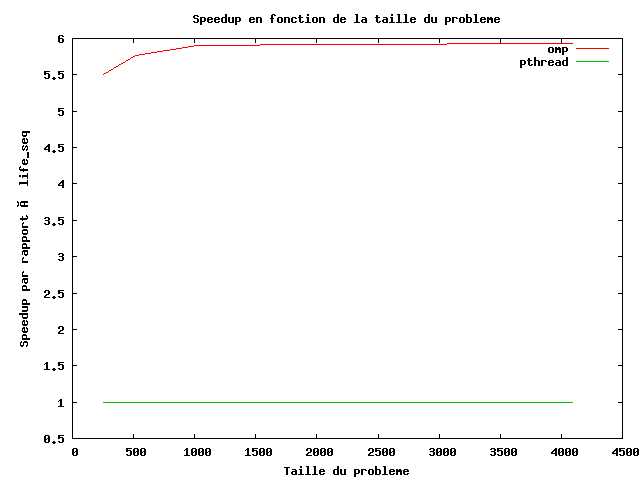
\includegraphics[scale=0.5]{single.png}
\caption{Speedups monoc\oe ur}
\label{fig:single}
\end{figure}

\newpage
\subsection{Implémentation MPI}

Le speedup de la version MPI, exécuté sur $4$ c\oe urs est une fonction constante en fonction de la taille de la grille initiale, égale environ à $4$ c'est-à-dire au nombre même de processus. Bien que ce speedup soit mesuré par rapport à la version exécutée sur $1$ c\oe ur (et non la version séquentielle), ce résultat  -- visible sur la figure \ref{fig:para} -- prouve que le jeu de la vie est extrêmement bien parallélisable puisqu'il permet d'atteindre le speed-up théoriquement maximal égal au nombre de processus mis en jeu. En ce qui concerne l'exécution sur $16$ c\oe urs, le speedup est cette fois-ci une courbe croissante (qui n'atteint qu'un speedup de $14$) en fonction de la taille de la grille. Cela peut s'expliquer par le trop grand nombre de communications induites pour la taille du problème : les calculs ne recouvrent les temps de communications qu'au fur et à mesure de l'augmentation de la taille des grilles locales au processus. Le speedup est toutefois supérieur à celui de l'exécution sur $4$ c\oe urs à partir d'une grille initiale de taille $1024$, et tend vers le maximum théorique de $16$ (il atteint $14$ pour une problème de taille $4096$ sur la figure \ref{fig:para}).

\begin{figure}[!h]
\centering
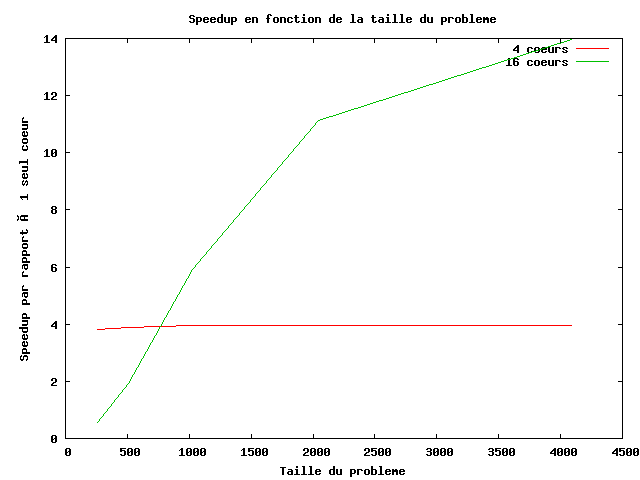
\includegraphics[scale=0.5]{para.png}
\caption{Speedups multic\oe ur}
\label{fig:para}
\end{figure}
\section*{Conclusion}
\addcontentsline{toc}{section}{Conclusion}

Nous regrettons fortement de ne pas avoir pu terminer toutes les implémentations, et de ne pas avoir fourni de benchmarks plus poussés. Cependant nous pensons que les objectifs minimaux sont atteints, et les résultats obtenus, bien que peu nombreux, sont en accord avec nos attentes.


\end{document}
